\documentclass[14pt, a4paper]{report}
\usepackage{mathtext}
\usepackage[T2A]{fontenc}
\usepackage[utf8]{inputenc}
\usepackage[russian]{babel}
\usepackage{multirow}
\usepackage{slashbox}
\usepackage{makecell}
\usepackage{graphicx}
\usepackage{physics}
\usepackage{amstext}
\usepackage{caption}
\usepackage{subcaption}
\usepackage{cmap}
\usepackage{float}
\usepackage{siunitx}

\renewcommand{\thesection}{\arabic{section}.}
\renewcommand{\thesubsection}{\arabic{section}.\arabic{subsection}.}

\title{\textbf{Отчет о выполнении лабораторной работы 4.1.1 "Геометрическая оптика"}}
\author{Алпатова Александра, Калашников Михаил, Б03-205}
\date{}

\begin{document}
\maketitle

\textbf{Цель работы:}
изучить методы определения фокусных расстояний линз и сложных оптических систем; определить характеристики оптической системы, составленной из тонких линз; изучить недостатки реальных линз -- сферическую и хроматическую аберрации.
\newline

\textbf{В работе используются:}
\begin{itemize}
\item оптическая скамья с набором рейтеров;
\item положительные и отрицательные линзы;
\item экран;
\item осветитель с ирисовой диафрагмой;
\item зрительная труба;
\item кольцевые диафрагмы;
\item линейка.
\end{itemize}

\section{Теоретические сведения}

\begin{figure}[H]
\centering
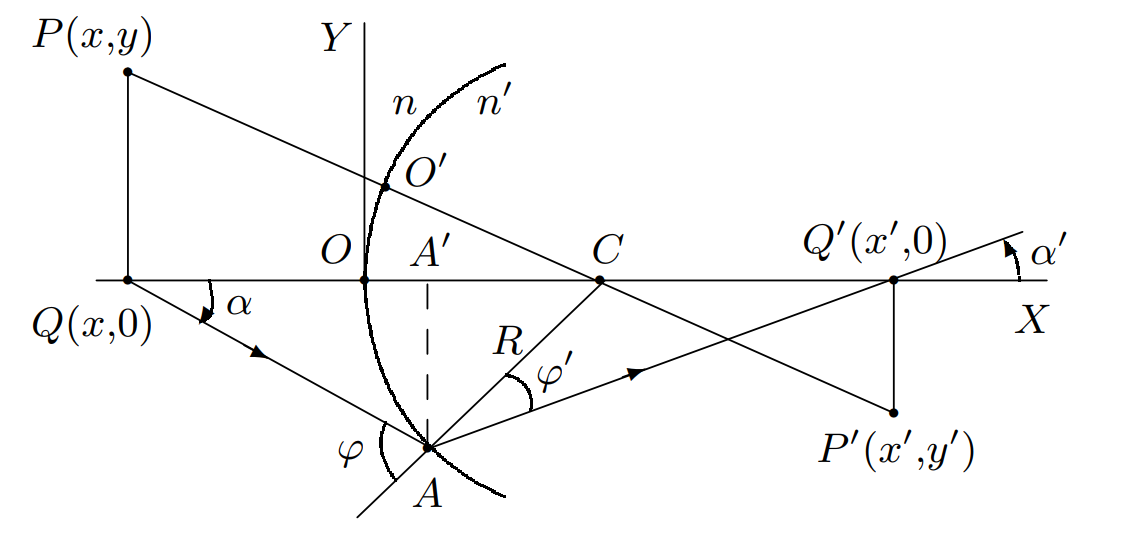
\includegraphics[width=0.8\linewidth]{../images/411_4}
\end{figure}

Используя закон преломления, получим для элементарной оптической ячейки, изображённой на рисунке выше, в параксиальном приближении:
\begin{equation}\label{опт-ячейка}
	-\frac{n}{x}+\frac{n'}{x'} = \frac{n'-n}{R},
\end{equation}
\begin{equation}
	x \alpha = x' \alpha'.
\end{equation}
Для прямой $ P P' $, рассмотренной как оптическая ось, 
\begin{equation}\label{PP}
	\frac{y'}{y} = \frac{x' - R}{x - R}.
\end{equation}

Проведя замену переменных, получим систему уравнений
\begin{equation}\label{grid}
	\frac{x' - F'}{H' - F'}= \frac{H-F}{x- F} = \frac{y'}{y} = \frac{n \alpha}{n' \alpha'},
\end{equation}
\begin{equation}\label{grid1}
	(x-H)\alpha= (x' - H')\alpha'.
\end{equation}
Из этих уравнений получим
\begin{equation}\label{Ф}
	\frac{n}{f} = -\frac{n'}{f'} \equiv \Phi,
\end{equation}
где
\begin{equation}\label{focus-len}
	f\equiv H - F, \;\;\; f'\equiv H' - F'.
\end{equation}
$ f $ и $ f' $ -- главные фокусные расстояния системы.

\section{Проведение эксперимента}

\begin{enumerate}

\item Изучим предоставленный набор из пяти линз и оценим их фокусные расстояния при помощи удаленного источника света.

\item Отцентрируем все элементы оптической системы.

\end{enumerate}

\subsection{Определение фокусных расстояний линз с помощью подзорной трубы}

\begin{enumerate}

\item Сфокусируем подзорную трубу на "бесконечность".

\item Расположим одну из линз на скамье, приблизительно на фокусном расстоянии. Перемещая линзу добьемся четкого изображения транспаранта источника.

\item Развернем линзу другой стороной и повторим измерения.

\item Проведем измерения несколько раз. Полученные значения занесем в таблицу.

\begin{table}[H]
\centering
\begin{tabular}{ccccc}
\hline
\multicolumn{1}{|c|}{n}          & \multicolumn{1}{c|}{1}  & \multicolumn{1}{c|}{2}   & \multicolumn{1}{c|}{3}   & \multicolumn{1}{c|}{4}   \\ \hline
\multicolumn{1}{|c|}{$f_a,\ мм$} & \multicolumn{1}{c|}{75} & \multicolumn{1}{c|}{126} & \multicolumn{1}{c|}{174} & \multicolumn{1}{c|}{241} \\ \hline
\multicolumn{1}{|c|}{$f_b,\ мм$} & \multicolumn{1}{c|}{79} & \multicolumn{1}{c|}{128} & \multicolumn{1}{c|}{178} & \multicolumn{1}{c|}{251} \\ \hline
\multicolumn{1}{l}{}             & \multicolumn{1}{l}{}    & \multicolumn{1}{l}{}     & \multicolumn{1}{l}{}     & \multicolumn{1}{l}{}    
\end{tabular}
\end{table}

\item Измерим случайную погрешность экспериментально: повторим одно измерение несколько раз и вычислим среднеквадратичное отклонение.

\begin{table}[H]
\centering
\begin{tabular}{|c|c|c|c|c|}
\hline
$f_{3a},\ мм$ & 177 & 175 & 177 & 176 \\ \hline
\end{tabular}
\end{table}

\[\sigma_{f,\ rand}=0.8\ мм\]

В качестве инструментальной погрешности возьмем цену деления линейки ($\sigma_{f,\ instr}=1\ мм$). Таким образом общая погрешность может быть вычислена по формуле:
\[\sigma_f=\sqrt{\sigma_{f,\ rand}^2+\sigma_{f,\ instr}^2}=1.3\ мм\]

\item Измерим фокусное расстояние отрицательной линзы. Получим, что $l=217\ мм$, $a_0=321\ мм$.
\[f_5=l-a_0=(-104\pm2.6)\ мм\]

\end{enumerate}

\subsection{Измерение фокусных расстояний линз по формуле тонкой линзы и методом Бесселя}

\begin{enumerate}

\item Выберем одну линзу и помести экран на некотором расстоянии от предмета.

\item Поместим исследую линзу между источником и экраном и найдем два положения, при которых возникают четкие действительные изображения.

\begin{table}[H]
\centering
\begin{tabular}{|c|c|c|c|c|}
\hline
n & $L,\ мм$  & $s1,\ мм$   & $s2,\ мм$  & $l,\ мм$    \\ \hline
1 & $556\pm2$ & $358\pm2.3$ & $228\pm2.3$ & $130\pm4.6$ \\ \hline
2 & $556\pm2$ & $360\pm2.3$ & $230\pm2.3$ & $130\pm4.6$ \\ \hline
\end{tabular}
\end{table}

\item Вычислим фокусные расстояния по формуле тонкой линзы:
\[\frac{1}{f}=\frac{1}{s}+\frac{1}{L-s}\]
и по приближенной формуле Бесселя:
\[f=\frac{L^2-l^2}{4L}\]

\begin{table}[H]
\centering
\begin{tabular}{|c|c|c|c|}
\hline
n & $f_{т.л.,\ a},\ мм$ & $f_{т.л.,\ б},\ мм$ & $f_{Б},\ мм$ \\ \hline
1 & $127\pm2$          & $135\pm2$           & $131\pm2$    \\ \hline
2 & $127\pm2$          & $135\pm2$           & $131\pm2$  \\ \hline
\end{tabular}
\end{table}

\end{enumerate}

\subsection{Измерение фокусных расстояний методом Аббе}

\begin{enumerate}

\item Установим линзу между осветителем с транспарантом и экраном.

\item Отодвинем осветитель на некоторое расстояние от линзы. Измерим новый размер изображения.

\item Рассчитаем фокусное расстояние линзы по методу Аббе:

\[f=\frac{\Delta x}{y_0/y_2-y_0/y_1}=(126\pm3)\ мм\]

\end{enumerate}

\subsection{Сборка и изучение подзорных труб Кеплера и Галилея}

\begin{enumerate}

\item Из имеющегося набора линз выберем три: две для телескопа и одну для коллиматора.

\item С помощью коллиматора создадим расположенный на бесконечности объект.

\item Глядя в окуляр вспомогательной подзорной трубы, оценик сколько ячеек сетки укладывается в поле зрения на размере окулярной риски.

\item Соберем на скамье модель телескопа Кеплера.

\item Измерим новый видимый размер изображения ячейки сетки осветителя. Рассчитаем увеличение и сравним его с теоретическим.

\begin{figure}[H]
\centering
\begin{minipage}{.5\textwidth}
  \centering
  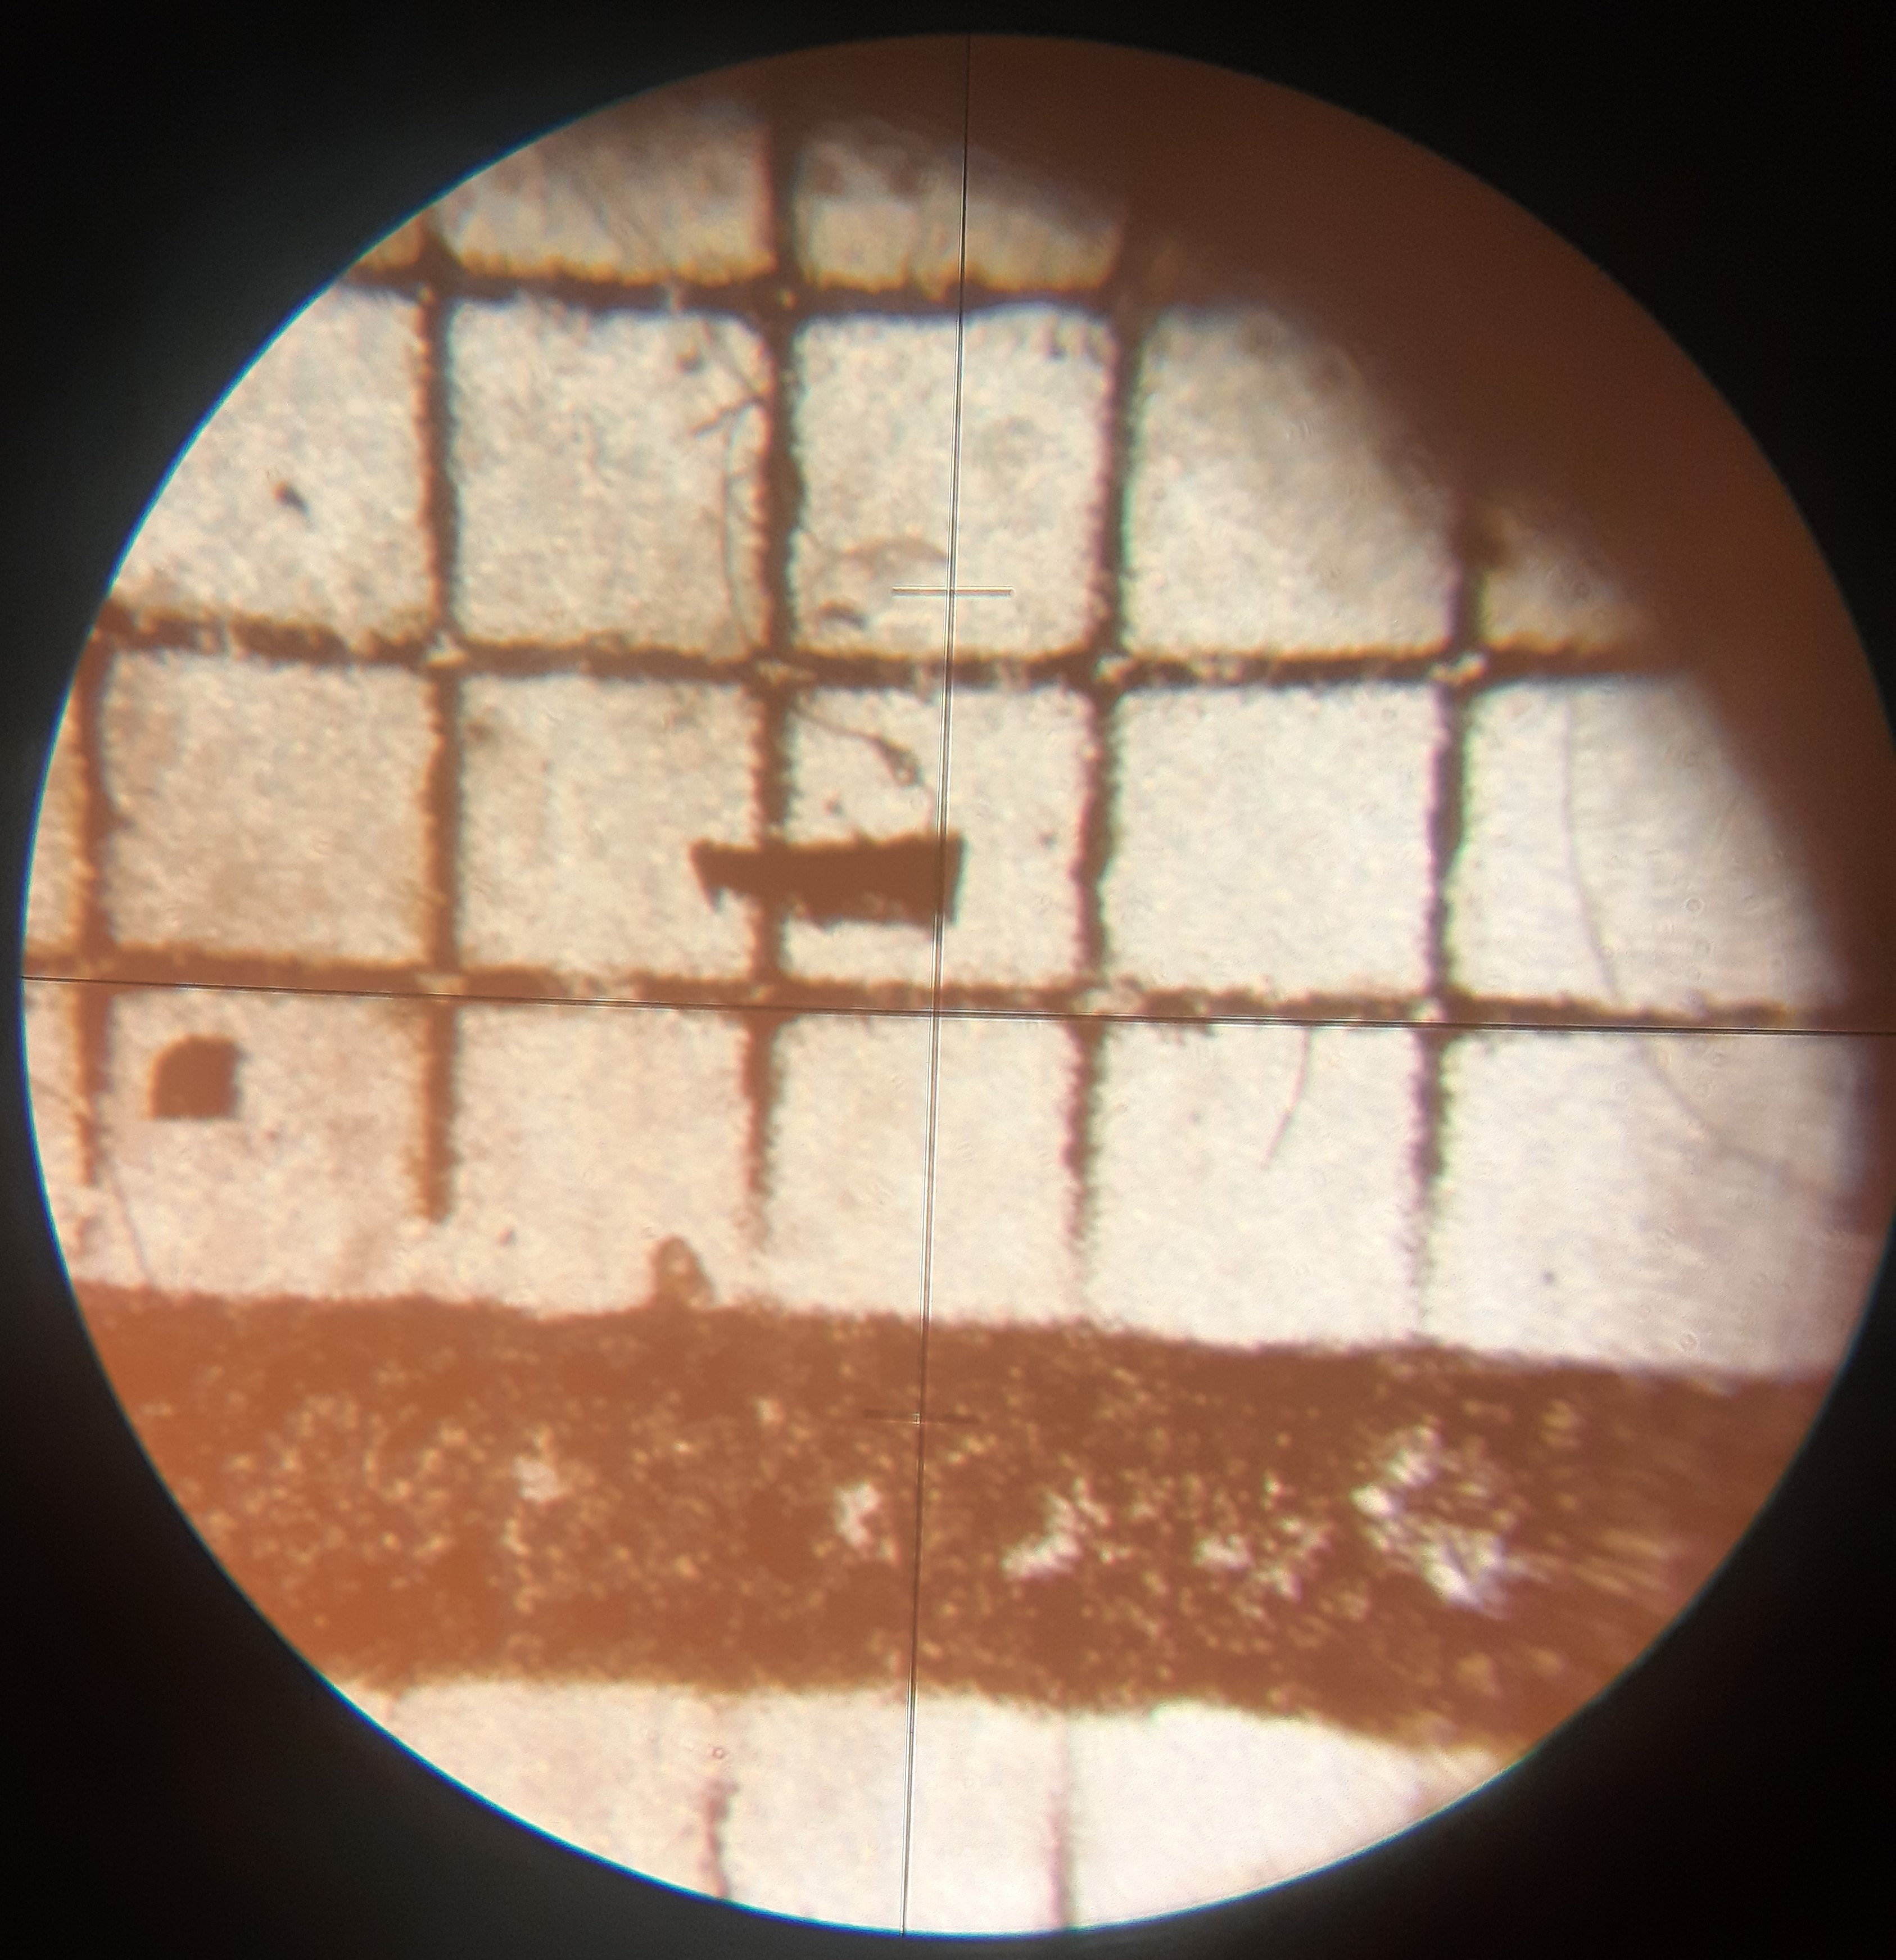
\includegraphics[width=.85\linewidth]{../images/411_1}
\end{minipage}%
\begin{minipage}{.5\textwidth}
  \centering
  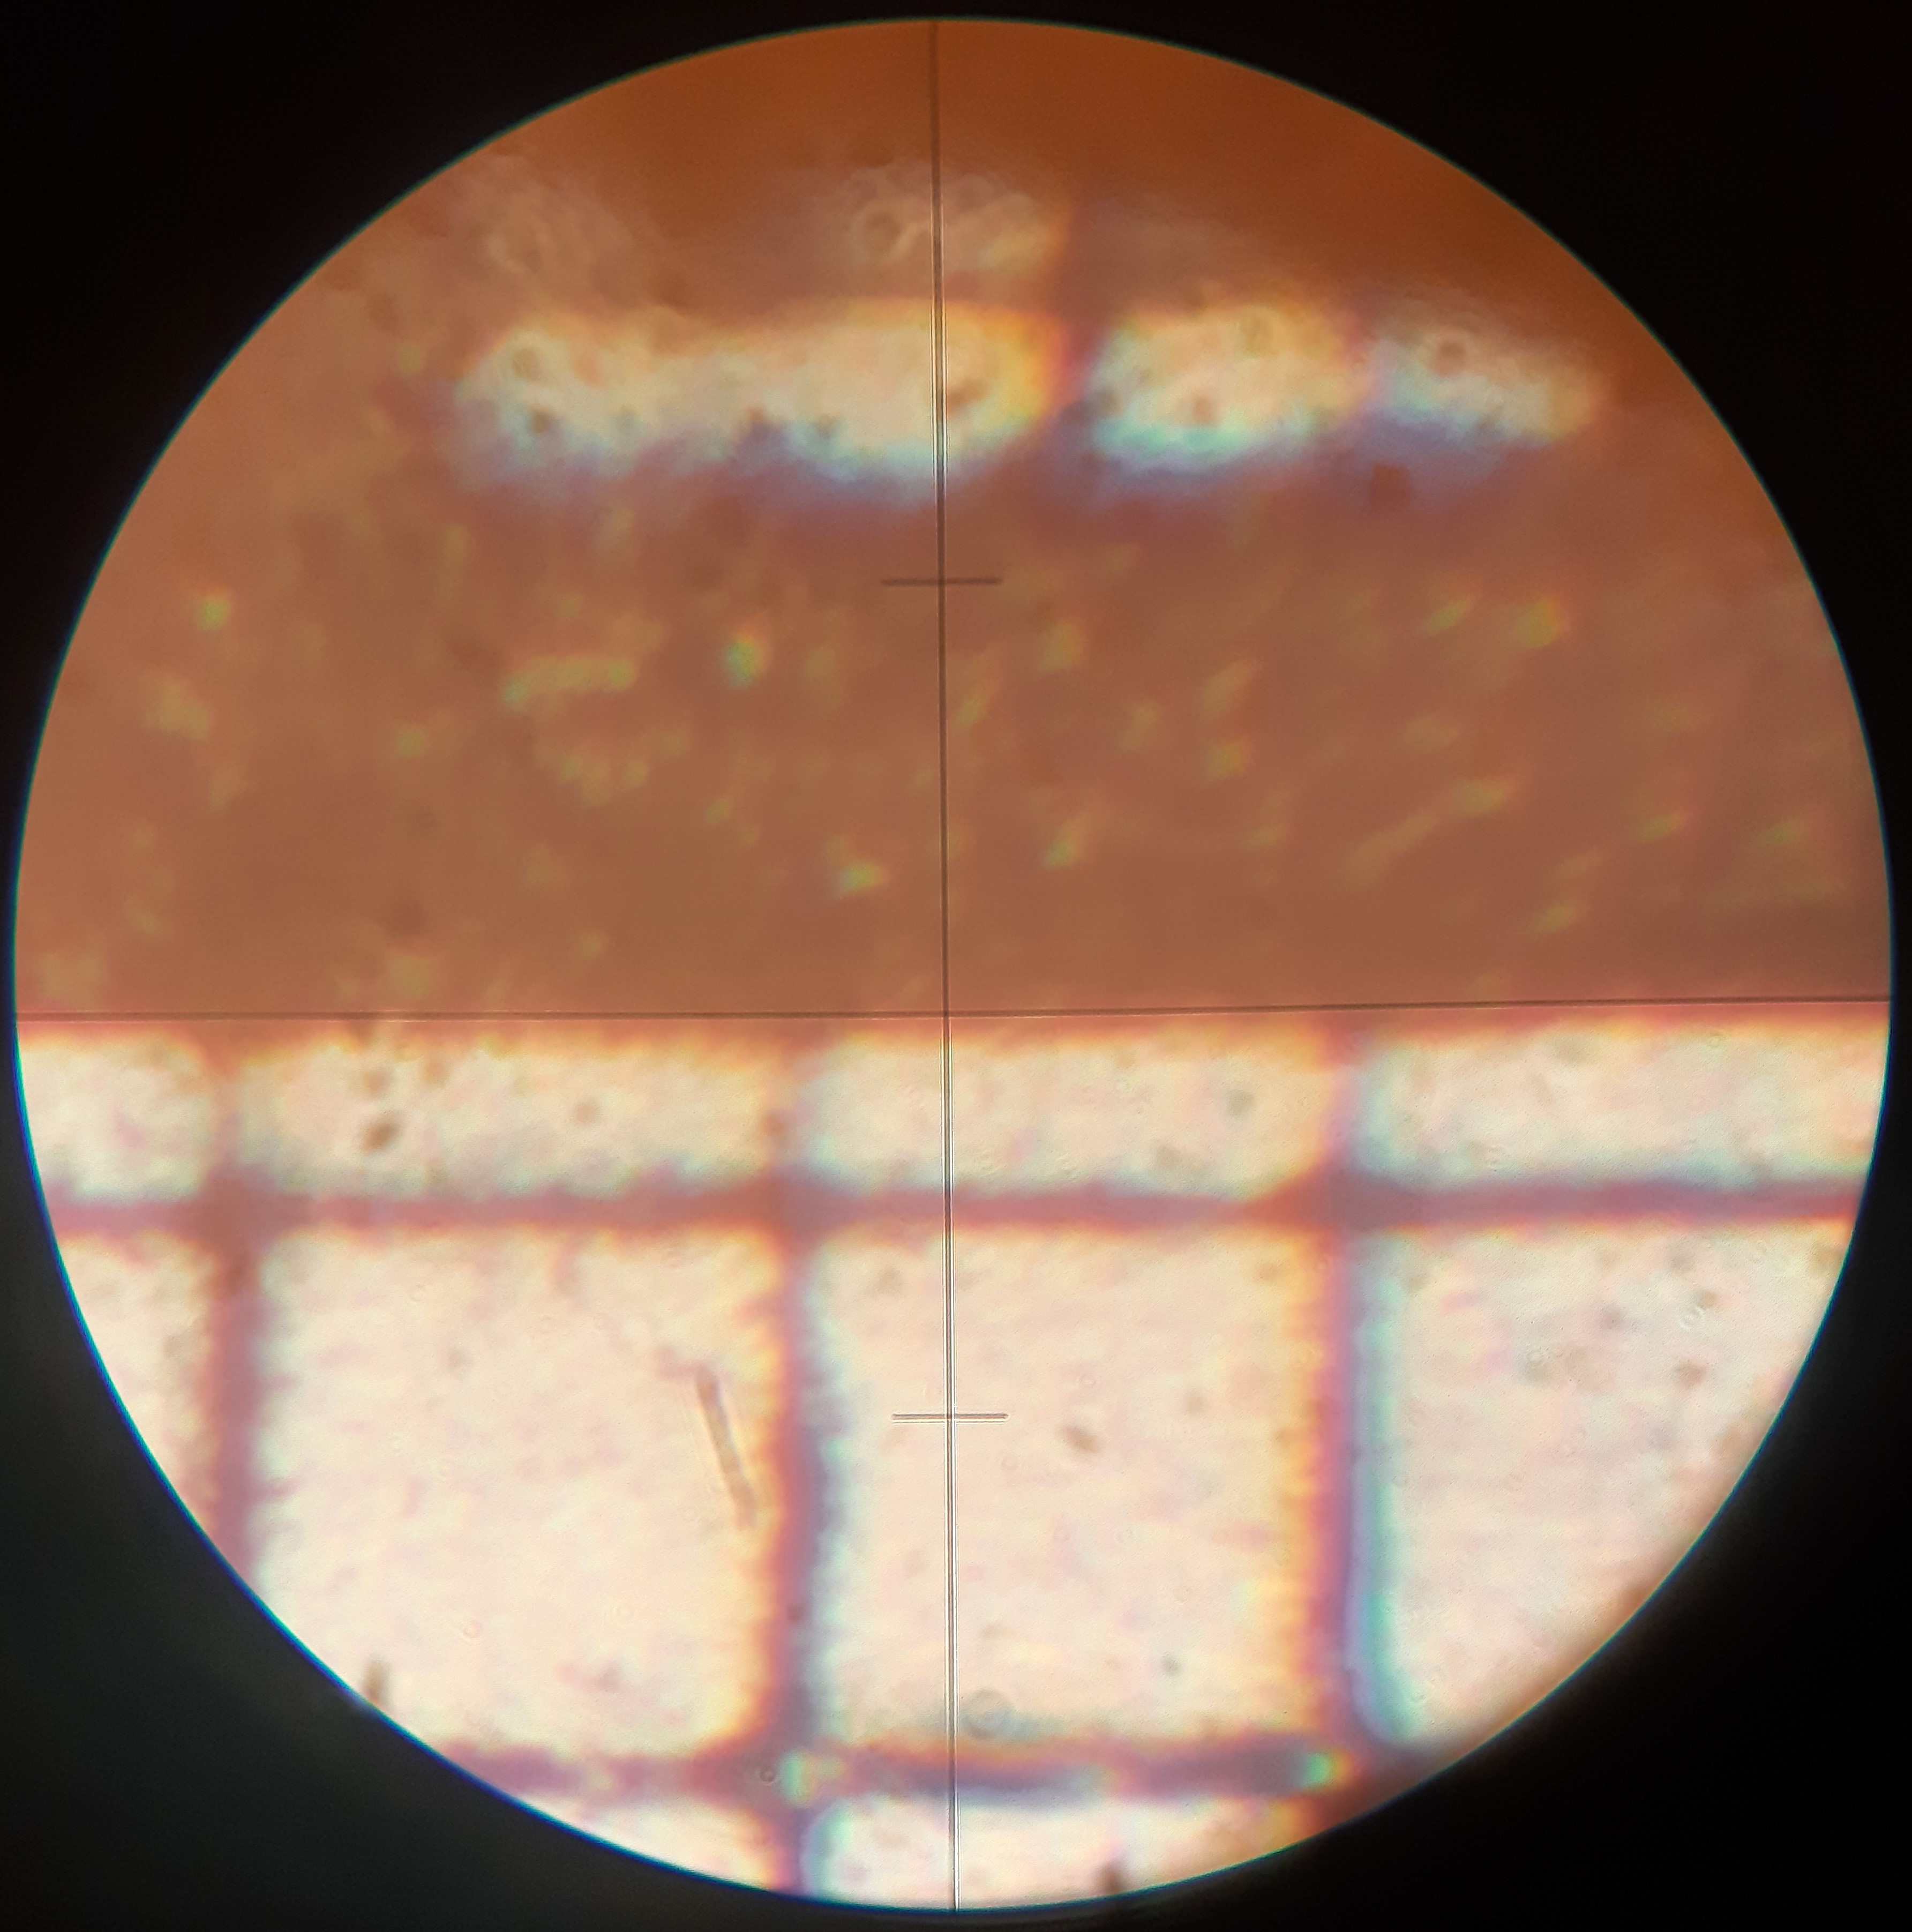
\includegraphics[width=.85\linewidth]{../images/411_2}
\end{minipage}
\end{figure}

\[\gamma=\frac{1.4}{0.8}\approx1.81\pm0.14\]

\end{enumerate}

\subsection{Сборка и изучение модели микроскопа}

\begin{enumerate}

\item Отберем из набора две короткофокусные линзы. Вычислим необходимую длину оптического интервала ($\gamma_\infty\approx4$, $L_{зр}\approx25\ см$):

\[\Delta=\gamma_\infty\frac{f_{об}f_{ок}}{L_{зр}}\approx15\ см\]

\item Разместим линзы на скамье согласно расчетам. Добьемся четкой фокусировки увеличенного изображения сетки.

\begin{figure}[H]
\centering
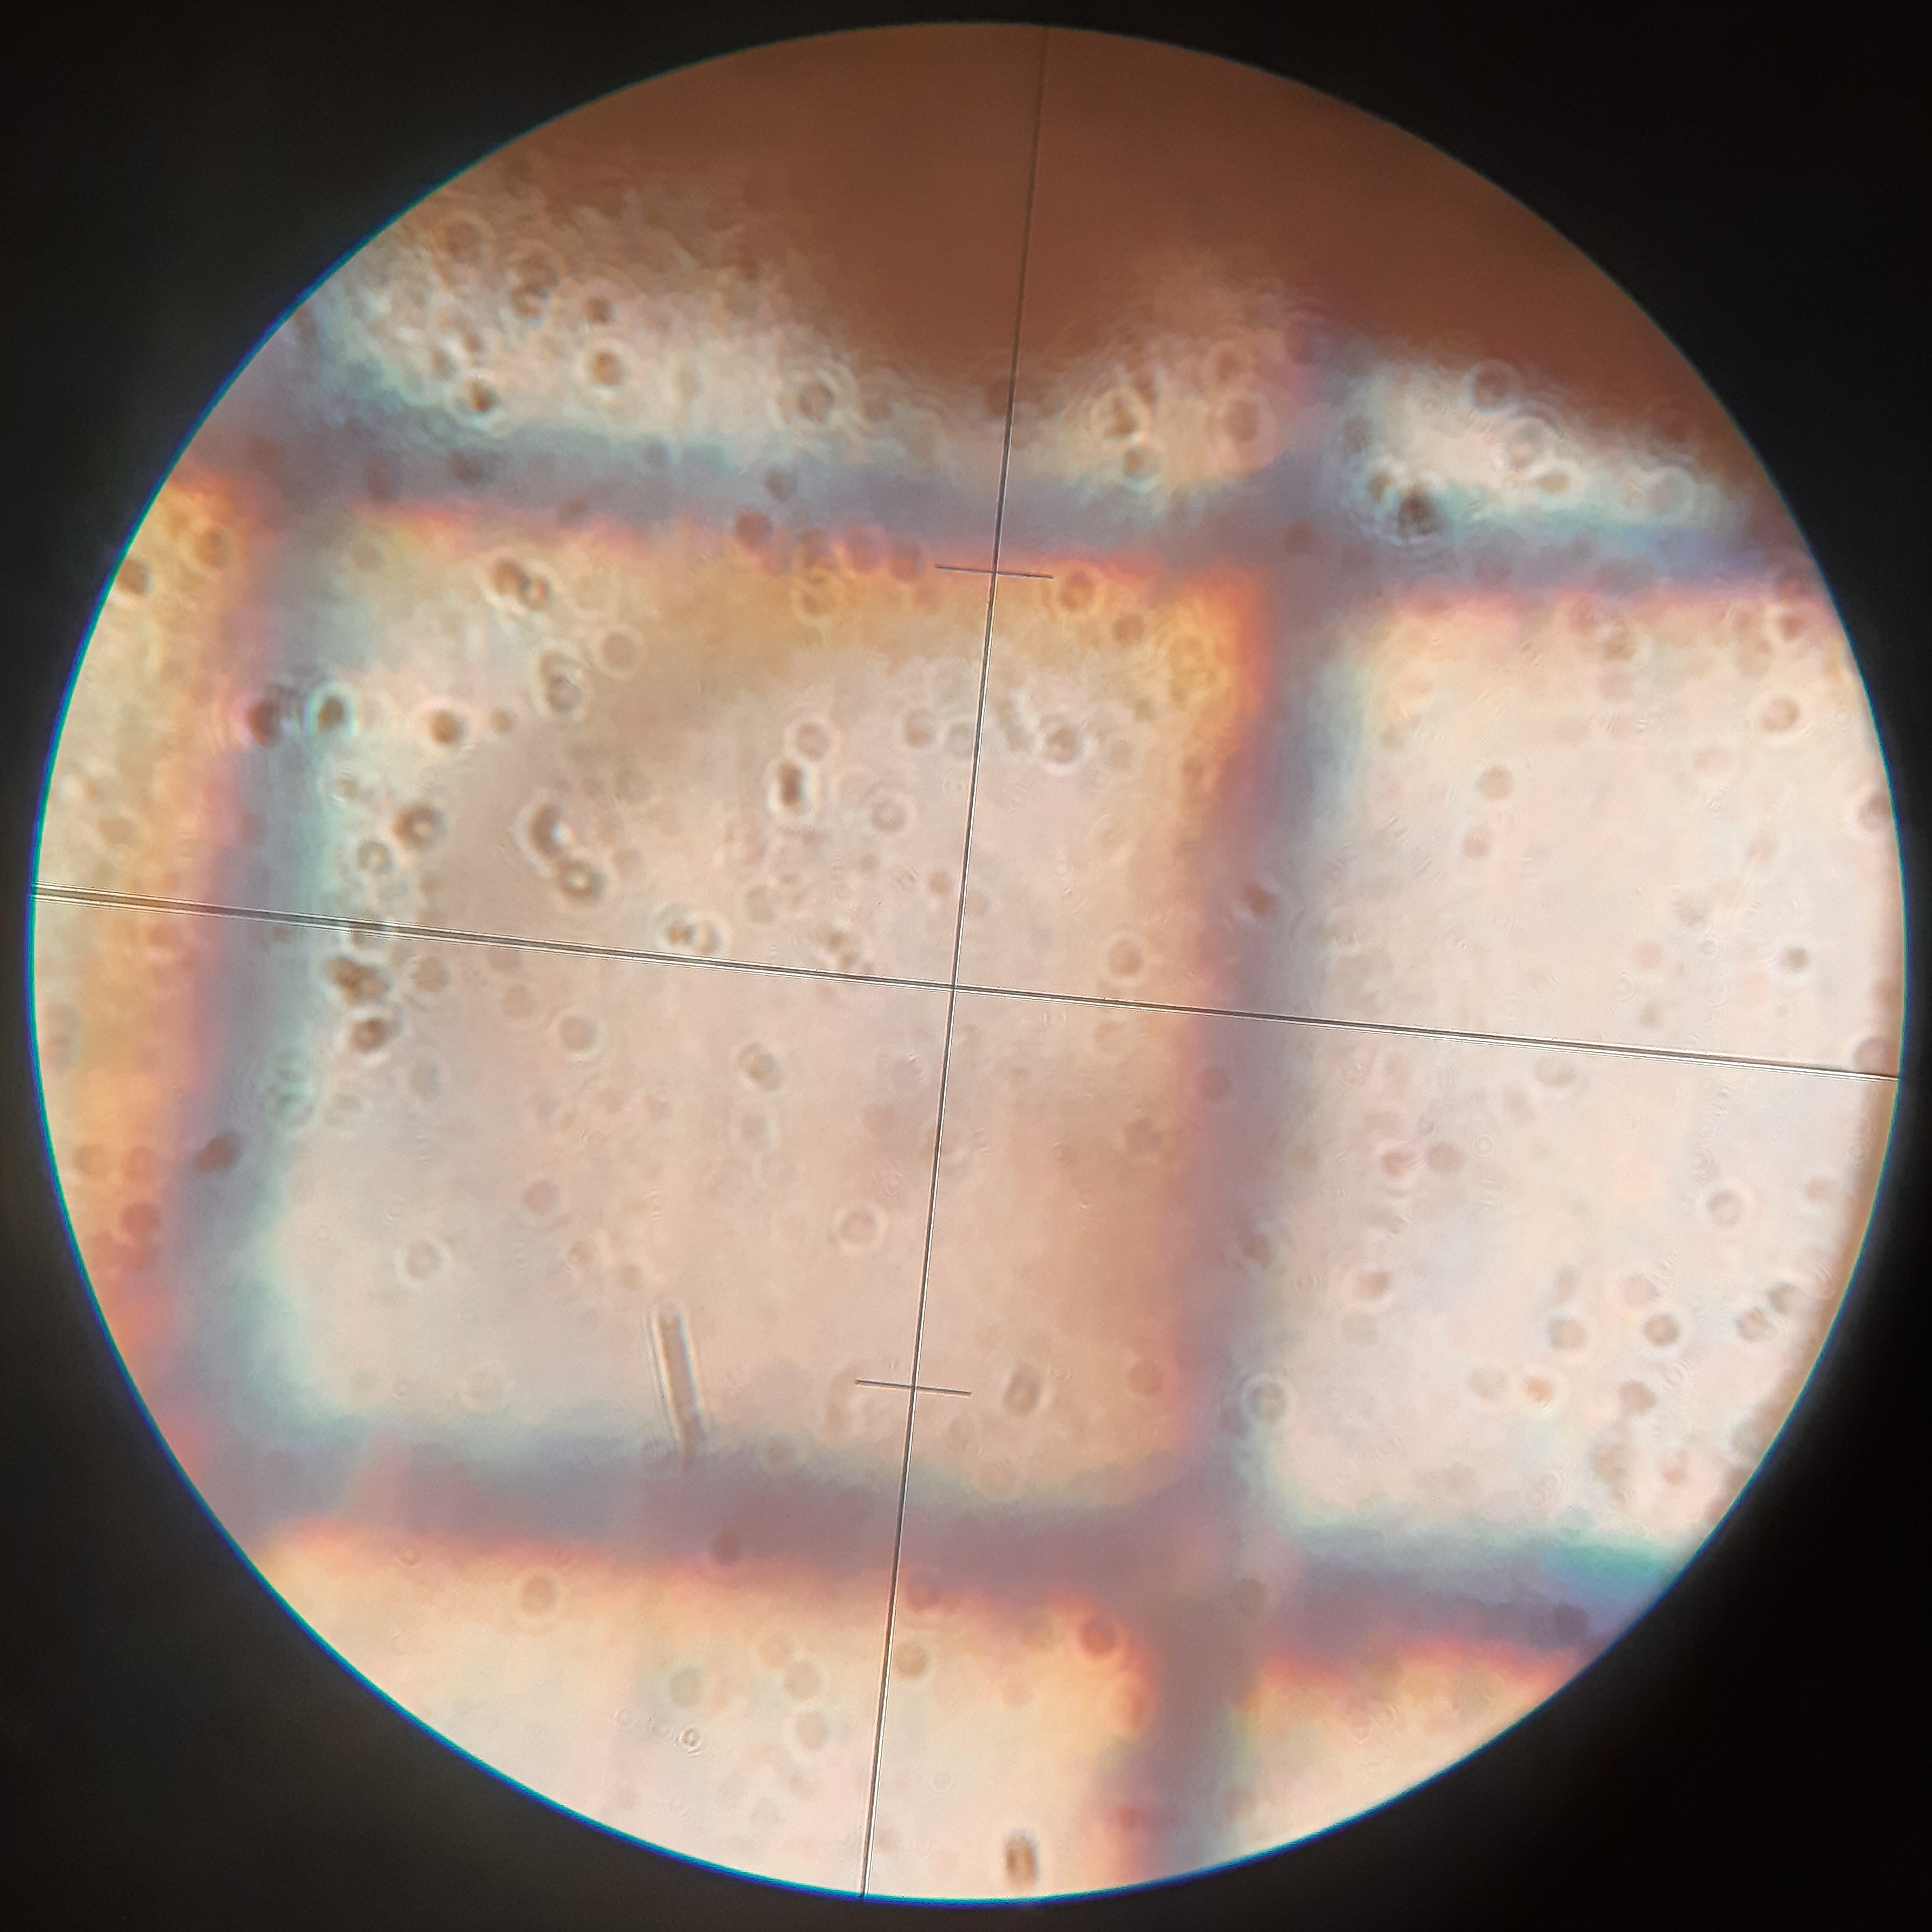
\includegraphics[width=.6\linewidth]{../images/411_3}
\end{figure}

\item Для измерения увеличения микроскопа воспользуемся настроенной на бесконечность вспомогательной трубой. В таком случае увеличение может быть вычислено по формуле:

\[\gamma_\infty=\frac{\alpha}{\alpha_0}\frac{L_{зр}}{f_{кол}}\approx3.3\pm0.2\]

\end{enumerate}

\section{Выводы}

В ходе работы были изучены методы определения фокусных расстояний линз. Также нам были определены характеристики оптической системы, составленной из тонких линз.

\end{document}